\chapter{Analysis}

Before going over the actual programming of the framework, we need to further inspect some of the features we have specified in the Introduction in Chapter \ref{Intro}. In this chapter, we will analyse features of this project, as well as suggest ways of solving problems, and in case there are more solutions, we will select the most suitable one with a proper explanation.


\section{Command System}


\section{Pathfinding}
In Requirement \ref{intro:req:pathfinding}  we have established that the player should have the ability to move around the map while avoiding obstacles. 
The development of the walking system could be divided into two main parts:
\begin{enumerate}
    \item The representation of the walkable map,
    \item The problem of finding the shortest path.
\end{enumerate} 

\subsection{Walkable Map}
One possible way of representing the walkable map would be to create a walkability bitmap. This bitmap would describe the possible walkable areas that the player may traverse. Figure \ref{fig:Bitmap} shows one such bitmap on top of the scene. The player is able to freely walk around the area highlighted with green color, while the dark areas are inaccessible. Finally, the player can step on the blue area only when certain conditions are met. 

\begin{figure}[H]
\centering
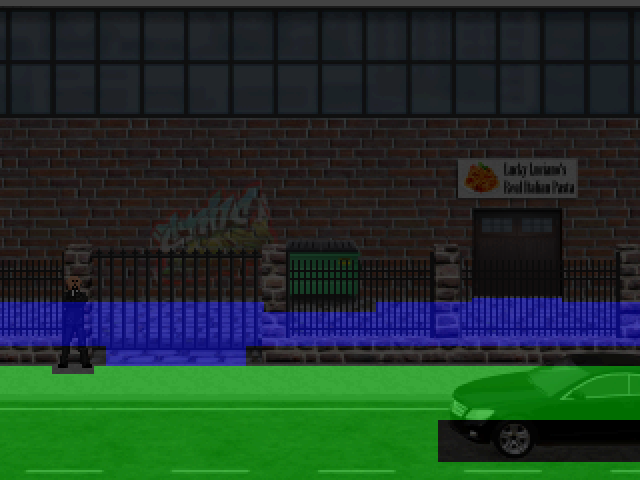
\includegraphics[width=.8\linewidth]{img/walkability.png}
\caption{Walkability bitmap. Source \cite{Shdon}.}
\label{fig:Bitmap}
\end{figure}

However, the user of the framework would most probably need to create this bitmap by themselves. In addition, modifying the bitmap is very difficult and time-consuming. Our aim is to make the experience user-friendly and this solution would go against that. 

The second and arguably more suitable approach enables us to create the map in the Unity Engine itself. To achieve this, the boundaries of the walkable map and obstacles must be defined. A map consisting of polygons offers itself as a solution to this problem, depicted in Figure. The user of the framework would be able to modify the shapes on the fly, making it easy to change the map even late in the development of the game. The idea is to have one primary polygon where characters and other interactable objects are located. Except for that, there are areas that the player cannot currently or indefinitely enter and these can be defined by an arbitrary number of polygons. 


\begin{figure}[H]
\centering
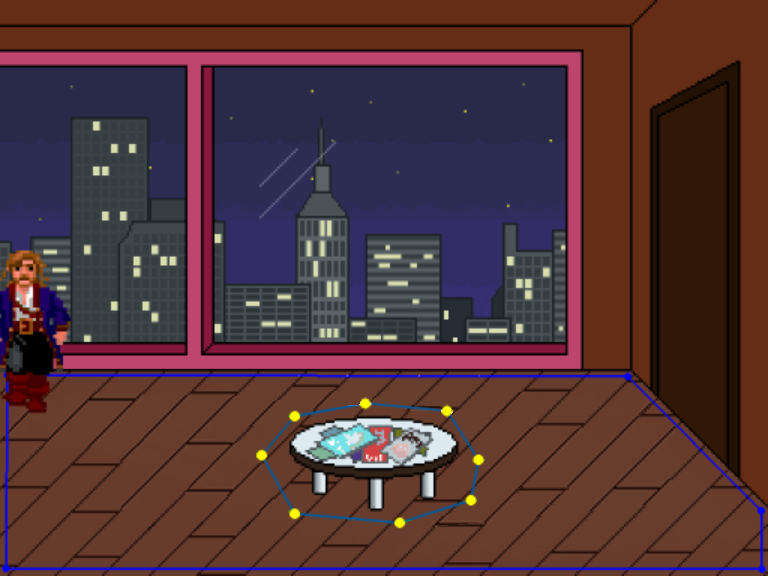
\includegraphics[width=.8\linewidth]{img/WS-polygons2.png}
\caption{Polygonal map. Source \cite{Uurloon1}.}
\label{fig:Bitmap}
\end{figure}

\subsection{Shortest path problem}
Naturally, we don’t want the character to wander aimlessly in search of the endpoint. The problem of finding the shortest path has been extensively researched, with many proven algorithms to solve it. One of the most widely used is the A* algorithm—a graph traversal and pathfinding method known for its efficiency. It is commonly applied in various fields of computer science, including game development, and is described in Algorithm \ref{alg:AStar}. 

\algrenewcommand\algorithmicrequire{\textbf{Input:}}
\algrenewcommand\algorithmicensure{\textbf{Output:}}
\renewcommand{\alglinenumber}[1]{#1.}

\begin{algorithm}
\caption{A* Search Algorithm}\label{alg:AStar}
\begin{algorithmic}[1]
\Require Start node $start$, Goal node $goal$
\Ensure Path from $start$ to $goal$ or failure
\Statex
\Function{A\_Star}{$start, goal$}
    \State $openList \gets \{start\}$
    \State $closedList \gets \emptyset$
    \State $start.g \gets 0$
    \State $start.h \gets \Call{Heuristic}{start, goal}$
    \State $start.f \gets start.g + start.h$
    \State $start.parent \gets null$
    \While{$openList \neq \emptyset$}
        \State $current \gets$ node in $openList$ with lowest $f$ value
        \If{$current = goal$}
            \State \Return \Call{Reconstruct\_Path}{$current$}
        \EndIf
        \State remove $current$ from $openList$
        \State add $current$ to $closedList$
        \For{each $neighbor$ of $current$}
            \If{$neighbor \in closedList$}
                \State \textbf{continue}
            \EndIf
            \State $tentative\_g \gets current.g + \Call{Distance}{current, neighbor}$
            \If{$neighbor \notin openList$}
                \State add $neighbor$ to $openList$
            \ElsIf{$tentative\_g \geq neighbor.g$}
                \State \textbf{continue}
            \EndIf
            \State $neighbor.parent \gets current$
            \State $neighbor.g \gets tentative\_g$
            \State $neighbor.h \gets \Call{Heuristic}{neighbor, goal}$
            \State $neighbor.f \gets neighbor.g + neighbor.h$
        \EndFor
    \EndWhile
    \State \Return failure
\EndFunction
\Statex
\Function{Reconstruct\_Path}{$current$}
    \State $path \gets \emptyset$
    \While{$current \neq null$}
        \State add $current$ to beginning of $path$
        \State $current \gets current.parent$
    \EndWhile
    \State \Return $path$
\EndFunction
\end{algorithmic}
\end{algorithm}

To use the A* algorithm, we first need a graph, so we must define one. A graph is a data structure consisting of nodes and the connections between them are defined by edges. However, in our case, creating a graph with all possible nodes and edges is unnecessary and even impractical—we need to filter out only the relevant information.

A node is included based on the shape and type of the corresponding polygon. In basic shapes like triangles, rectangles and squares, any two points can be connected by a straight line without encountering obstacles. However, if the walkable area is concave (containing one or more nodes with interior angles greater than 180 °), some vertices point inward, creating obstructions that block direct visibility between points, which is depicted in Figure \cite{Polygons}. To account for these obstructions, a node is added to the graph only if its vertex is concave. Convex vertices have an interior angle that is no more than 180 ° and are therefore excluded as they do not create any obstacles. Regarding edges, an edge is included in the graph only if the two nodes that form it are within each other’s line of sight.


\begin{figure}[H]
\centering
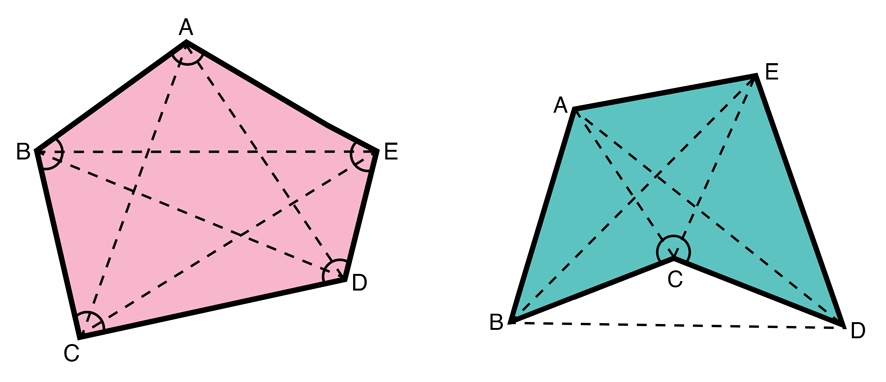
\includegraphics[width=.8\linewidth]{img/polygons.png}
\caption{Convex (left) and concave (right) polygons. Source \cite{Polygons}.}
\label{fig:Polygons}
\end{figure}


The situation is reversed for obstacles (meaning non-main polygons) as we do not want to stay inside these obstacles but on the outside. Since we need to go around them, in this case we take into account convex vertices instead of concave ones. Here, the concave vertices do not stand in the way of two points, but the convex ones do. 

A key component of the A* algorithm is the heuristic function which estimates the cost of the cheapest path to the goal. If the function never overestimates it, A* is guaranteed to return one of the shortest paths from start to goal. Common heuristic functions satisfying this condition include the Manhattan distance and the Euclidean distance. For the purpose of free character movement on a 2D plane, the Euclidean distance was chosen as a heuristic function. It can be calculated from the Cartesian coordinates of the points while also applying the Pythagorean theorem:

\[
d = \sqrt{(x_2 - x_1)^2 + (y_2 - y_1)^2}
\]

\section{Depth Simulation}
As we have specified in Requirements \ref{intro:req:scale} and \ref{intro:req:layers}, we want to simulate the feeling of a 3D space.

by dynamically scaling the character as well as adjusting the layer order of objects.

\subsection{Scaling}
Firstly, we will look closely at character scaling. 

\subsection{Layering}
Next, let us examine the layering. Our aim is to dynamically adjust the visibility of objects, as seen in Figure \ref{fig:Layers}. Because we are working with a 2D space, we have to do a bit more work determining in what order the sprites of objects should be displayed. Fortunately, it is very simple to do since all we need is to look at the Y coordinates. If object A has a smaller Y coordinate than object B, it means that A should be drawn on top of B. 


\begin{figure}[H]
\centering
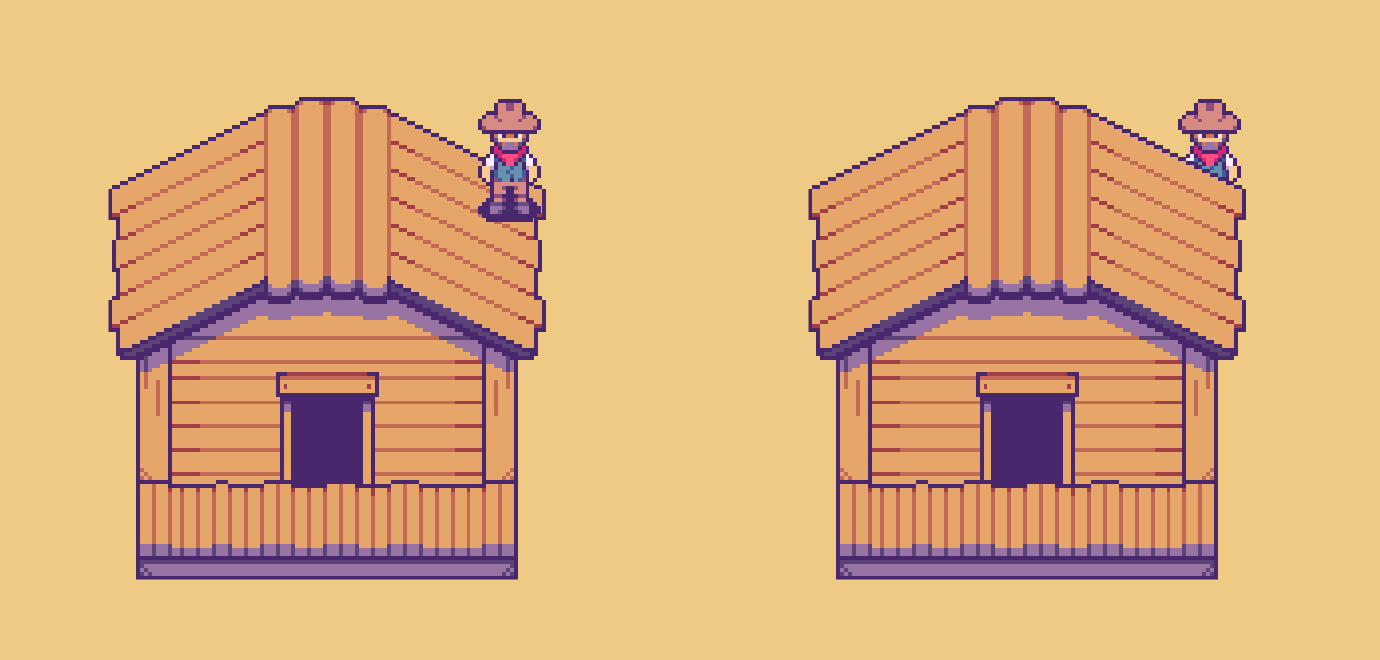
\includegraphics[width=.8\linewidth]{img/layers.png}
\caption{Wrong (left) and correct (right) layer ordering. Source \cite{Piotr}.}
\label{fig:Layers}
\end{figure}

\section{Inventory System}


\section{Dialogue System}


